%%%%%%%%%%%%%%%%%%%%%%%%%%%%%%%%%%%%%%%%%%%%%%%%%%%%%%%%%%%%%%%%%%%%%%%%%%%%%%%%
\documentclass[twocolumn]{revtex4}

%%%%%%%%%%%%%%%%%%%%%%%%%%%%%%%%%%%%%%%%%%%%%%%%%%%%%%%%%%%%%%%%%%%%%%%%%%%%%%%%
% Note that comments begin with a "%" and are not turned into text in the .pdf
% document.
%%%%%%%%%%%%%%%%%%%%%%%%%%%%%%%%%%%%%%%%%%%%%%%%%%%%%%%%%%%%%%%%%%%%%%%%%%%%%%%%

%%%%%%%%%%%%%%%%%%%%%%%%%%%%%%%%%%%%%%%%%%%%%%%%%%%%%%%%%%%%%%%%%%%%%%%%%%%%%%%%
% Include some extra packages.
%%%%%%%%%%%%%%%%%%%%%%%%%%%%%%%%%%%%%%%%%%%%%%%%%%%%%%%%%%%%%%%%%%%%%%%%%%%%%%%%
\usepackage[]{graphicx}
%%%%%%%%%%%%%%%%%%%%%%%%%%%%%%%%%%%%%%%%%%%%%%%%%%%%%%%%%%%%%%%%%%%%%%%%%%%%%%%%

%%%%%%%%%%%%%%%%%%%%%%%%%%%%%%%%%%%%%%%%%%%%%%%%%%%%%%%%%%%%%%%%%%%%%%%%%%%%%%%%
\begin{document}

%%%%%%%%%%%%%%%%%%%%%%%%%%%%%%%%%%%%%%%%%%%%%%%%%%%%%%%%%%%%%%%%%%%%%%%%%%%%%%%%
\title{
Journal article
}

\author{M. Harrison}
\affiliation{Siena College, Loudonville, NY}

\date{\today}

\begin{abstract}
	The goal of this experiment is to calculate probability of rainfall in a month using lists of random numbers in Python. This method is the Monty Carlo method.
A lot of the information that should be in this document is not, because I ran out of time to complete the project. 
	



\end{abstract}

\maketitle
%%%%%%%%%%%%%%%%%%%%%%%%%%%%%%%%%%%%%%%%%%%%%%%%%%%%%%%%%%%%%%%%%%%%%%%%%%%%%%%%

%%%%%%%%%%%%%%%%%%%%%%%%%%%%%%%%%%%%%%%%%%%%%%%%%%%%%%%%%%%%%%%%%%%%%%%%%%%%%%%%
\section{Introduction}
This project used the Monty Carlo method of using random numbers to approximate the probability of certain amounts of rainfall in a month. This was an assignment for CSIS 200: Software Tools for Physicists at Siena College. The Monte Carlo method used involved generating a large number of hypothetical months, and in those months, thirty random numbers were generated. If those numbers were within the given probability, it would rain on that day.
%%%%%%%%%%%%%%%%%%%%%%%%%%%%%%%%%%%%%%%%%%%%%%%%%%%%%%%%%%%%%%%%%%%%%%%%%%%%%%%%


%%%%%%%%%%%%%%%%%%%%%%%%%%%%%%%%%%%%%%%%%%%%%%%%%%%%%%%%%%%%%%%%%%%%%%%%%%%%%%%%
\section{Approach and Results}

 With this method, I discovered that the probability it would rain on only one day in a month if each day had a 20\% chance of rain was 0.93\%, verified by the mathematical expression for this probability, $30*(0.2*0.8^{29})$. The approach used hundreds of thousands of generated months in a for loop in python and made a list of how many of those months would have one day of rain, based on whether or not the random number assigned to a given day using numpy.random.random was less than 0.2. The amount of months added to that list was then divided by the total number of generated months to find the probability.

The determined probability of it raining on 8 days in a month in any order was determined to be 0.7\%, also found with the Monte Carlo Method. This test used the same method, but used 10\% as the probability of rain on a given day, and counted how many months had at least 8 days of rain.

In the third problem, the probability was given for certain amounts of rainfall and depended on whether or not it rained on previous days. To find the amount of rain fall in a month, I again used a for loop to generate a number of months, then looped again through the 30 days in each month. For each of those days, if the probability was such that it would rain, it appended to a list the amount of rain that probability implies would fall. Then, it would proceed to a nested conditional for the probability of it raining the next day. The amount of months that would have more than ten centimeters or more of rain were counted and divided by the total number of months in the initial loop to calculate the probability of there being more than ten centimeters of rain in a month. The probability found was 33\%.

\begin{figure}
 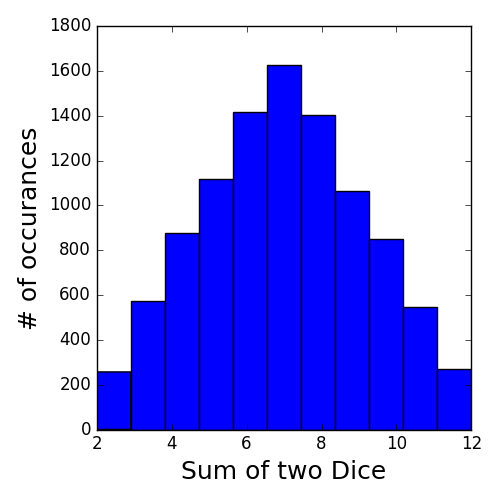
\includegraphics[width=0.45\textwidth]{histo.png}
\caption{This is from the dice simulation, since I was having serious problems trying to graph my results}
\end{figure}
%%%%%%%%%%%%%%%%%%%%%%%%%%%%%%%%%%%%%%%%%%%%%%%%%%%%%%%%%%%%%%%%%%%%%%%%%%%%%%%%

%%%%%%%%%%%%%%%%%%%%%%%%%%%%%%%%%%%%%%%%%%%%%%%%%%%%%%%%%%%%%%%%%%%%%%%%%%%%%%%%
\end{document}
%%%%%%%%%%%%%%%%%%%%%%%%%%%%%%%%%%%%%%%%%%%%%%%%%%%%%%%%%%%%%%%%%%%%%%%%%%%%%%%%
